\documentclass[a4paper,12pt]{article}
%%%%%%%%%%%%%%%%%%%%%%%%%%%%%%%%%%%%%%%%%%%%%%%%%%%%%%%%%%%%%%%%%%%%%%%%%%%%%%%%%%%%%%%%%%%%%%%%%%%%%%%%%%%%%%%%%%%%%%%%%%%%%%%%%%%%%%%%%%%%%%%%%%%%%%%%%%%%%%%%%%%%%%%%%%%%%%%%%%%%%%%%%%%%%%%%%%%%%%%%%%%%%%%%%%%%%%%%%%%%%%%%%%%%%%%%%%%%%%%%%%%%%%%%%%%%
\usepackage{eurosym}
\usepackage{vmargin}
\usepackage{amsmath}
\usepackage{graphics}
\usepackage{enumerate}
\usepackage{framed}
\usepackage{epsfig}
\usepackage{subfigure}
\usepackage{fancyhdr}

\setcounter{MaxMatrixCols}{10}
%TCIDATA{OutputFilter=LATEX.DLL}
%TCIDATA{Version=5.00.0.2570}
%TCIDATA{<META NAME="SaveForMode" CONTENT="1">}
%TCIDATA{LastRevised=Wednesday, February 23, 2011 13:24:34}
%TCIDATA{<META NAME="GraphicsSave" CONTENT="32">}
%TCIDATA{Language=American English}

\pagestyle{fancy}
\setmarginsrb{20mm}{0mm}{20mm}{25mm}{12mm}{11mm}{0mm}{11mm}
\lhead{MA4128} \rhead{Mr. Kevin O'Brien}
\chead{Advanced Data Modelling}
%\input{tcilatex}

\begin{document}
	\section*{Testing Model Assumptions: Tutorial Sheet}


\begin{enumerate}


\item 
Numeric Transformations, such as logarithmic transformation, are often used in statistical analysis as an approach for dealing with non-normal data.
\begin{itemize}
	%	\item[(i)] (1 Marks) Discuss the importance of numeric transformations, such as logarithmic transformation, in Statistics.
	%	\item[(ii)] Describe the process of transformations
	\item[(i.)] (1 Mark) Describe the purpose of Tukey's Ladder (referencing direction and relative strength).
	\item[(ii.)] (2 Marks) Give two examples of a transformation for various types of skewed data (i.e. an example for both types of skewness).
	\item[(iii.)] (1 Mark) Discuss the limitations of numeric transformations.
\end{itemize}
\bigskip

\item 
The typing speeds for one group of 12 Engineering students were recorded both at the beginning of year 1 of their studies. The results (in words per minute) are given below:

\begin{center}
	\begin{tabular}{|c|c|c|c|c|c|}
		\hline
		% Subject& A& B& C& D& E &F &G &H \\ \hline
		149  & 146 & 112 & 142 & 168& 153\\ \hline
		137 & 161 & 156& 165&  170&  159
		\\ \hline
	\end{tabular}
\end{center}
Use the Dixon Q-test to determine if the lowest value (118) is an outlier. You may assume a significance level of 5\%.
\begin{itemize}
	\item[(i.)](1 Mark)	State the Null and Alternative Hypothesis for this test.
	\item[(ii.)](2 Marks) Compute the test statistic
	\item[(iii.)](1 Mark) State the appropriate critical value.
	\item[(iv.)](1 Mark) What is your conclusion to this procedure.
\end{itemize}

%============================%
\item \textbf{Outliers}
\begin{itemize}
	\item[(i.)] (3 Marks) Provide a brief description for three tests from the family of Grubb's  Outliers Tests. Include in your description a statement of the null and alternative hypothesis for each test
	\item[(ii.)] (2 Marks) Describe any required assumptions for tests, and the limitations of these tests.
\end{itemize}
% Part A - Dixon Q Test (5 Marks)
\item Use the Dixon Q-test to determine if there is an outlier present in this sample data. You may assume
a significance level of 5\%.
\[ 131, 136, 103, 117, 123, 127, 122, 132, 135\]
\begin{enumerate}[(i)]
	\item (1 Mark) State the null and alternative hypotheses for this test.
	\item (2 Marks) Compute the test statistic?
	\item (1 Mark) State the appropriate critical value.
	\item (1 Mark) What is your conclusion to this procedure?
\end{enumerate}

\newpage

\item Suppose that the results of an experimental procedure resulted in the collection of datasets $X$. Consider the following inference procedure performed on data set $X$.
\begin{center}
	\begin{framed}
		\begin{verbatim}
		> shapiro.test(X)
		
		Shapiro-Wilk normality test
		
		data:  X
		W = 0.9619, p-value = 0.6671
		
		\end{verbatim}
	\end{framed}
\end{center}


\begin{itemize}
	\item[(i)] (1 Mark) Describe the purpose of this procedure.
	\item[(ii)] (1 Mark) What is the null and alternative hypothesis?
	\item[(iii)] (1 Mark) What is your conclusion about this procedure?
\end{itemize}
\item 
A graphical procedure was carried out to assess whether or not this assumption of normality is valid for data set \texttt{Y}. Consider the Q-Q plot in the figure below.

\begin{center}
	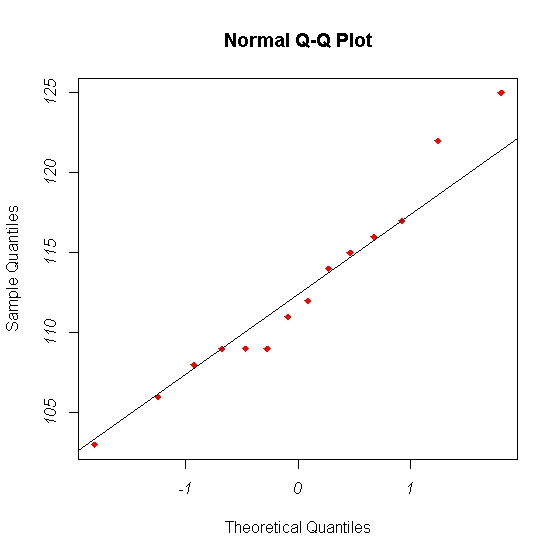
\includegraphics[scale=0.55]{images/Q5examQQplot}
\end{center}

\begin{itemize}
	\item[(iv)] (1 Mark) Provide a brief description on how to interpret this plot.
	\item[(iv)] (1 Mark) What is your conclusion for this procedure? Justify your answer.
\end{itemize}

\end{enumerate}

\end{document}
